\documentclass{article}
\usepackage[french]{babel}
\usepackage[utf8]{inputenc}
\usepackage{ansmath}
\usepackage{amssymb}
\usepackage{amsmath}
\usepackage[fleqn]{nccmath}
\usepackage{listings}
\usepackage{graphicx}
\allowdisplaybreaks

\title{TP d'Analyse Scilab}

\author{
    Carre Ludovic
    \and
    Carlin Cyril
}


\begin{document}
\maketitle

\section{Exercice 1}
On obtient z = 0 et w = 1. Pourtant d'un point de vue formelle, l'addition étant associative, z = w.
Cela s'explique du fait que la différence entre y et x est inférieur à $2,2*10^{16}$.
Par conséquent, étant donné que la machine calcule en premier la valeur de la parenthèse, on a :  
\begin{displaymath}
    y - x \approx -x \\
    \Leftrightarrow
    z \approx 0
\end{displaymath}
Cependant, pour w,
\begin{eqnarray*}
    x - x &\approx& 0\\
    \Rightarrow
    w &\approx& y / y\\
    \Rightarrow
    w &\approx& 1
\end{eqnarray*}

\section{Exercice 2}
\begin{figure}[h]
\noindent 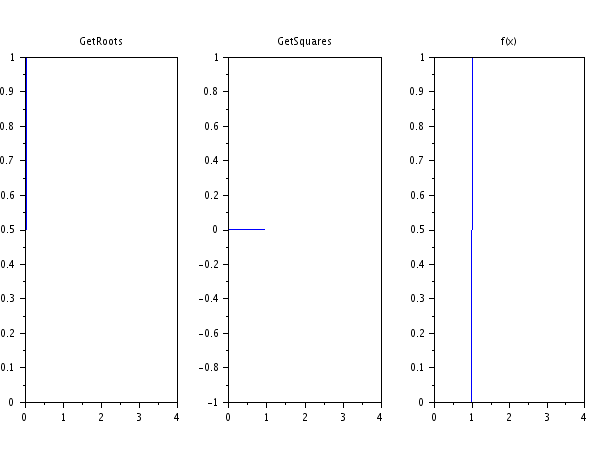
\includegraphics[width=\linewidth]{ImgExercice2.png}
\end{figure}
Mathématiquement, f(x) devrait se comporter comme la fonction identité f: x${->}$x définie sur [0;4] en l'occurrence. Or la courbe que l'on observe n'est définie que sur [0;1] et elle s'approche de la droite x=1.\\Ceci est dû au comportement de la fonction GetSquares, si x est supérieur à 1 la valeur de x$^{128}$ n'est pas représentable, le résultat de ce calcul sur Scilab est inf. Si x est inférieur à 1, la valeur de x$^{128}$ est représenté par 0. Enfin, si x=1 la valeur de x$^{128}$ est égale à 1.\\\\
Donc seules les valeurs inférieurs ou égales à 1 sont représentables par GetSquares. De plus, pratiquement tous les y de GetRoots sont égaux à 1 car il s'agit de la valeur représentable la plus proche du résultat exacte. Tous les x sont donc égaux à 1, ces informations nous permettent de comprendre le résultat observé.

\section{Exercice 3}
    \begin{enumerate}
        \item Pour obtenir la relation de récurrence sur cette suite d'intégrale, on effectue  un intégration par partie afin de descendre le degré de x : 
            \begin{displaymath}
                \forall n \in \mathbb{N}\ \ I_{n+1} = \int_{0}^1 x^{n+1}e^{x}dx
                                    = [x^{n+1}e^x]-(n+1)\int_{0}^1 x^{n}e^{x}dx
                                    = e - (n+1)I_n
            \end{displaymath}
            De plus
            \begin{displaymath}
                I_0 = e - 1
            \end{displaymath}
            On obtient donc la relation de récurrence suivante :
            \begin{displaymath}
                \left\{
                \begin{array}{rcr}
                    I_{n+1} & = & e - (n+1)I_n \\
                    I_0 & = & e - 1 \\
                \end{array}
                \right.
            \end{displaymath}
            La relation de récurrence n'étant pas linéaire (présence de n dans la relation), il faut donc intuiter une expression de $I_{n}$ en fonction de n à partir des premiers termes : 
            \begin{displaymath}
                \forall n \in \mathbb{N}   I_n = (-1)^{n}n!(e\sum_{k=1}^{n} \frac{(-1)^{k}}{k!} + I_0)
            \end{displaymath}
            On montre alors aisément par récurrence que cette expression est correcte à partir de la relation obtenue ci-dessus.
            D'où
            \begin{displaymath}
                I_{20} = 20!(e\sum_{k=1}^{20} \frac{(-1)^{k}}{k!} + I_0)
            \end{displaymath}
            Grâce à un algorithme simple, on calcule alors $I_{20}$ sur Scilab. On obtient
            \begin{displaymath}
                I_{20} \approx -1.693.10^{37}
            \end{displaymath}
            Ce résultat est absurde. D'une part il est négatif alors que $I_{20}$ est l'intégrale d'une fonction positive sur l'intervalle [0,1], donc par positivité de l'intégration $I_{20}$ est également positif. D'autre part,             
            \begin{eqnarray*}
                \forall x \in [0,1]  &0 \leq x^{20}e^{x} \leq e \\ 
                \text{Donc par croissance de l'intégration,} &0 \leq I_{20} \leq e
            \end{eqnarray*}

            Cette abération est dû à l'approximation de la machine sur la valeur de e. En effet, Scilab possède une valeur de e précise à $10^{-16}$ près. Or, la présence de n! dans l'expression de $I_{n}$ rend cette précision insuffisante pour le $20^{e}$ rang.
            Il faut donc trouver une autre méthode pour calculer cette intégrale de sorte à minimiser la propagation de l'incertitude sur la valeur de e.

    \item On rappelle le développement en série entière de $e^{c}$ : 
        \begin{displaymath}
            e^{x} = \sum_{n=0}^{\infty} \frac{x^n}{n}
        \end{displaymath}
        Donc en remplaçant dans $I_{20}$, on obtient 
        \begin{eqnarray*}
            I_{20} & =&  \int_{0}^1 x^{20}\sum_{n=0}^{\infty} \frac{x^n}{n}dx \\
                   & =&  \sum_{n=0}^{\infty} \frac{1}{n!}\int_{0}^1 x^{20+n}dx \ \ \text{car $\sum_{n=0}^{\infty} \frac{x^{20+n}}{n!}$ converge uniformément (cf série exponentielle)} \\
                   & =&  \sum{n=0}^{\infty} \frac{1}{n! (21+n)} \\
                   & \approx&  0,12380
        \end{eqnarray*}

    \item L'approximation faite en utilisant le DSE est plus précise que la méthode récursive qui propage et amplifie l'erreur d'approximation faite sur e. Ce résultat est cohérent car le DSE utilise une approximation polynomiale qui est mieux gérée par Scilab. En effet, si l'on calcule la série exponentielle, on s'aperçoit qu'au bout de 50 termes la valeur donné par cette somme est déjà plus précise que la valeur de e retenue par Scilab.
        
\end{enumerate}

\section{Exercice 4}
La méthode des rectangles permet de calculer une valeur approchée de l'intégrale d'une fonction. Deux fonctions ont été codées sur Scilab: SquareMethod(f,a,b,n) et I(x) afin d'implémenter cette méthode.
Le résultat renvoyé par SquareMethod(I,0,1,100000) est assez proche du résultat obtenue à l'exercice précédent. La méthode des rectangles n'est cependant pas la plus précise. La méthode des trapèzes et celle de Simpson donnent des résultats plus proche de la réalité:
\begin{displaymath}
    Rectangles: 0.1237902398291272354491.
\end{displaymath}
\begin{displaymath} 
    Trapezes: 0.1238038312382695321778.
\end{displaymath}
\begin{displaymath}
    Simpson: 0.1238038307625704548265.
\end{displaymath}
Nous pouvons cependant encore rapprocher le résultat de la méthode des rectangles en rajoutant des points, on obtient ainsi avec n=1000000:\\
\begin{displaymath}
    Rectangles: 0.1238024716264136543265.
\end{displaymath}

\section{Exercice 5}
On rappelle la définition de la fonction f, définie sur [-$\frac{1}{2}$,$\frac{1}{2}$] :
\begin{equation}
        \label{f} 
    f(x) = 
    \left\{
        \begin{array}{lll} 
                    -1 & \text{pour} & -\frac{1}{2} \le x \le 0 \,,\\ 
                    1 & \text{pour} & 0< x < \frac{1}{2} \,.
        \end{array}
    \right.
\end{equation}
On peut tout de suite remarquer que la fonction f est impaire, ce qui implique par définition de $a_n$ et $b_n$ que $a_n = 0$ (intégration d'une fonction impaire sur une période). On pourra donc se contenter de calculer les coefficients $b_n$ pour obtenir la série de fourier de f dans son intégralité.
\begin{eqnarray*}
    \forall n \in \mathbb{N}\ b_n &=& 2\int_{-0,5}^{0,5} f(t)sin(2\pi nt)dt\\
                                  &=& 2(\int_{-0,5}^0 -sin(2\pi nt)dt +\int_{0}^{0,5} sin(2\pi nt)dt\\
                                  &=& 2(\frac{(-1)^{n+1}+1}{2\pi n} + \frac{1+(-1)^{n+1}}{2\pi n})\\
                                  &=& 2\frac{(-1)^{n+1}+1}{n\pi}
\end{eqnarray*}
Donc la série de fourier associé à f s'écrit : 
\begin{eqnarray*}
    f(x) &=& \sum_{n=1}^{\infty} 2\frac{(-1)^{n+1}+1}{n\pi}sin(2\pi nx)\ \ \text{Or}\ \forall n \equiv 0 [2]\  b_n=0\\
         &=& \sum_{n=0}^{\infty} \frac{4}{\pi} \frac{sin(2(2n+1)\pi x)}{n}\\
         &=& \frac{4}{\pi}\sum_{n=0}^{\infty} \frac{sin(2(2n+1)\pi x)}{n}
\end{eqnarray*}
On remarque que cette formule est valide sur $\mathbb{R}$-$\left . -0.5,0,0.5\right .$ , c'est-à-dire là où f est continue.

\section{Exercice 6}
Le programme suivant permet de calculer la série de Fourier tronquée de la fonction f définit dans l'exercice 5. Pour ce faire on utilise la formule 6 de l'exercice précédent et on calcul la somme partielle des n premiers termes.
\noindent 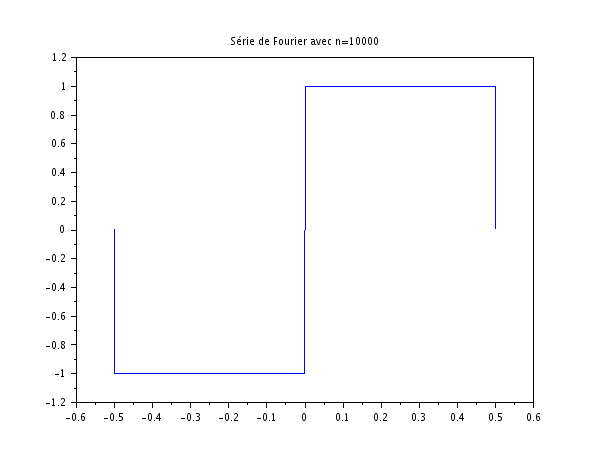
\includegraphics[width=\linewidth]{ImgExercice6.png}
Le comportement de la fonction est bien celui auquel nous nous attendions. On observe sur le graphe que la série de Fourier ne concorde pas avec la définition de la fonction f en x $\in{-1/2,0,1/2}$.\\
\noindent 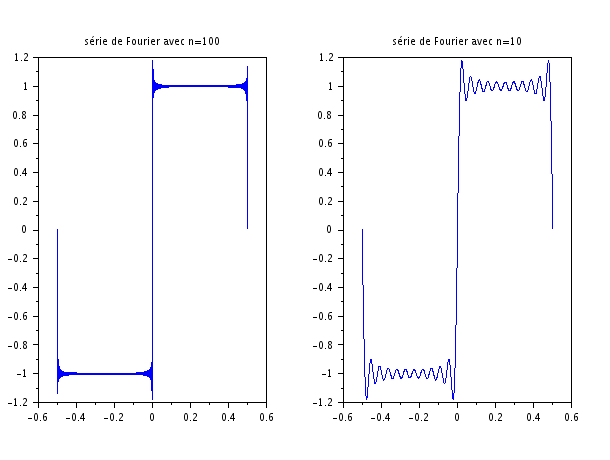
\includegraphics[width=\linewidth]{Img2Exercice6.png}
Plus n est grand plus la fonction est plate entre ]-1/2;0$[$ et ]0;1/2$[$, plus n est petit plus elle oscille entre ces intervales. Ceci est cohérent car plus on augmente n, plus on se rapproche de la série de Fourier qui converge vers f.
Comme la série de Fourier associée à f converge vers celle-ci exceptée en {-0.5,0,0.5}, soit un nombre fini de points, on peut affirmer que la série de Fourier converge presque partout vers f.

\section{Exercice 7}
\begin{enumerate}
   \item
	\begin{align*}
		&D_k = {z \in \mathbb{C} / |z-a_{kk}| \leq \sum_{j=1,j\neq k}^N |a_{kj}| = \Gamma_{k}}
	\end{align*}
Soit $\lambda \in$ Sp(A)
\begin{flalign*}
	&\exists v \neq 0\ tel\ que\ Av = \lambda v &&\\
	&\Leftrightarrow \forall k \in [1,N] \sum_{j=1}^N a_{kj}v_k = \lambda v_k&&\\
	&\Leftrightarrow \forall k \in [1,N] \sum_{j=1,j\neq k}^N a_{kj}v_k = (\lambda - a_{kk})v_k&&\\
	&\Leftrightarrow \forall k \in [1,N]\ |\lambda - a_{kk}| \leq \sum_{j=1,j\neq k}^N |a_{kj}v_k|\ \text{Par inégalité triangulaire}&&\\
	&\Leftrightarrow \forall k \in [1,N]\ |\lambda - a_{kk}|*|v_k| \leq (\sum_{j=1,j\neq k}^N |a_{kj}|)*|v_k|&&\\	
	&\text{Comme par définition d'un vecteur propre, v $\neq$ 0, alors $\exists k_0 \in$ [1,N] tq $v_{k_0} \neq 0$}&&\\
	&\Rightarrow |\lambda - a_{k_0k_0}| \leq \sum_{j=1,j\neq k_0}^N |a_{k_0j}|&&\\
	&\Rightarrow \lambda \in D_{k_0}&&
\end{flalign*}

    \item Graphe Scilab                                    
	\begin{figure}[h]
	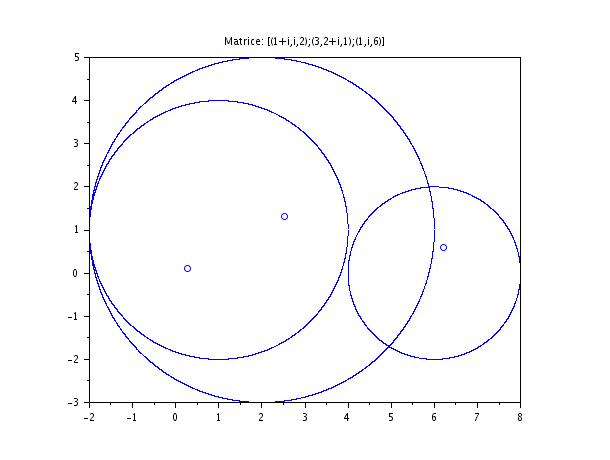
\includegraphics[width=\linewidth]{ImgExercice7.png}
	\end{figure}
    \item 	
	Cf.le fichier Scilab joint.
On a bien chaque valeur propre de la matrice qui est contenu dans un des disques de Gerschg\"orin.

	    \item
	Supposons par l'absurde que A est une matrice à diagonale dominante et non inversible.\\
	Comme A n'est pas inversible, 
	\begin{flalign*}
		&\exists v \in ker(A), v \neq 0\ tel\ que\ Av = 0\\
		&\Leftrightarrow 0 \in Sp(A)\\
		&\Rightarrow \exists i \in [1,N]\ tel\ que\ 0 \in D_i\\
		&\Rightarrow |0-a_{ii}| \leq \sum_{k \neq i}^N |a_{ik}|\\
		&\Rightarrow |a_{ii}| < |a_{ii}|\ \text{car A est à diagonale dominante}\\
	\end{flalign*}
	Ceci est absurde. Donc A est 0 $\in$ Sp(A), c'est-à-dire, A est inversible.
	
\end{enumerate}

\end{document}
